\documentclass[border=0cm]{standalone}
\usepackage{tikz}
\usetikzlibrary{arrows, arrows.meta}
\tikzset{    
    barbarrow/.style={ % style that just defines the arrow tip
        >={Straight Barb[left,length=5pt,width=5pt]},
        thick,
        <->
    },
    blues/.style={
        color=blue
    },
    reds/.style={
        color=red
    }
}
\definecolor{light-gray}{gray}{0.9}

\begin{document}
\begin{tabular}{@{}c@{}}
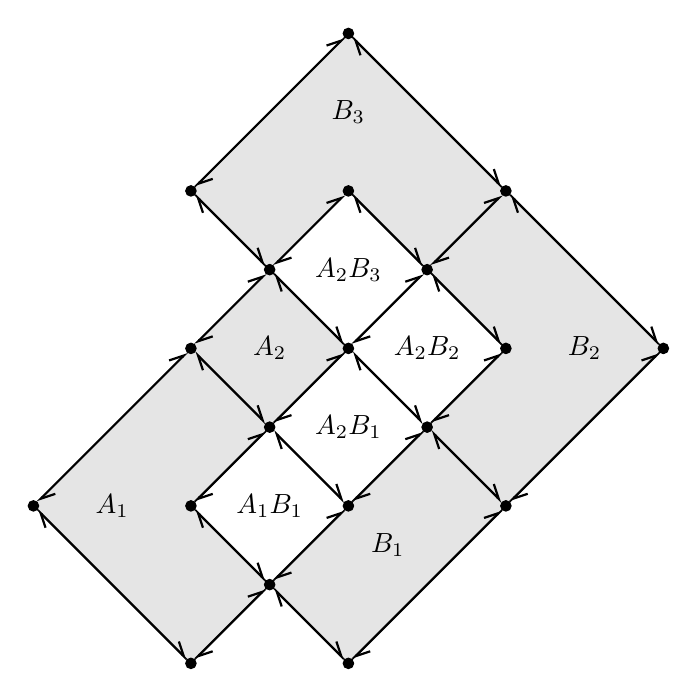
\begin{tikzpicture}
    \tikzstyle{node1}=[draw,scale=0.4,shape=circle,color=black,fill=black]
    %\draw[color=light-gray, style=dashed] (0,0) grid (8,8);

    \draw[fill=light-gray] (3,5) -- (2,6) -- (4,8) -- (8,4) -- (4,0) -- (3,1) -- (6,4) -- (4,6) ;
    \draw[fill=light-gray] (0,2) -- (2,0) -- (3,1) -- (2,2) -- (4,4) -- (3,5);
    
    \node[node1=A] (A) at (0,2) {};    \node[node1=C] (C) at (2,0) {};
    \node[node1=D] (D) at (2,2) {};    \node[node1=E] (E) at (2,4) {};
    \node[node1=F] (F) at (2,6) {};    \node[node1=G] (G) at (3,1) {};
    \node[node1=H] (H) at (3,3) {};    \node[node1=I] (I) at (3,5) {};
    \node[node1=J] (J) at (4,0) {};    \node[node1=K] (K) at (4,2) {};
    \node[node1=L] (L) at (4,4) {};    \node[node1=M] (M) at (4,6) {};
    \node[node1=N] (N) at (4,8) {};    \node[node1=O] (O) at (5,3) {};
    \node[node1=P] (P) at (5,5) {};    \node[node1=Q] (Q) at (6,2) {};
    \node[node1=R] (R) at (6,4) {};    \node[node1=S] (S) at (6,6) {};
    \node[node1=T] (T) at (8,4) {};

    \node at (1,2)    {$A_1$};
    \node at (7,4)    {$B_2$};
    \node at (4,7)    {$B_3$};
    \node at (4.5,1.5){$B_1$};
    \node at (3,2)    {$A_1B_1$};
    \node at (4,3)    {$A_2B_1$};
    \node at (3,4)    {$A_2$};
    \node at (5,4)    {$A_2B_2$};
    \node at (4,5)    {$A_2B_3$};
    
    
    \draw[barbarrow] (A) -- (C);\draw[barbarrow] (A) -- (E);
    \draw[barbarrow] (C) -- (G);\draw[barbarrow] (D) -- (G);
    \draw[barbarrow] (D) -- (H);\draw[barbarrow] (E) -- (H);
    \draw[barbarrow] (E) -- (I);\draw[barbarrow] (F) -- (I);
    \draw[barbarrow] (F) -- (N);\draw[barbarrow] (G) -- (J);
    \draw[barbarrow] (H) -- (L);\draw[barbarrow] (I) -- (L);
    \draw[barbarrow] (I) -- (M);\draw[barbarrow] (J) -- (Q);
    \draw[barbarrow] (G) -- (K);\draw[barbarrow] (H) -- (K);
    \draw[barbarrow] (K) -- (O);\draw[barbarrow] (L) -- (O);
    \draw[barbarrow] (L) -- (P);\draw[barbarrow] (M) -- (P);
    \draw[barbarrow] (N) -- (S);\draw[barbarrow] (O) -- (Q);
    \draw[barbarrow] (O) -- (R);\draw[barbarrow] (P) -- (R);
    \draw[barbarrow] (P) -- (S);\draw[barbarrow] (Q) -- (T);
    \draw[barbarrow] (S) -- (T);
\end{tikzpicture}
\end{tabular}
\end{document}
